\section{Projeto de Extensão CInovação Social}
\label{cinovacaosocial}

O projeto CInovação Social foi concebido visando a prática da Inovação Social Aberta por meio da Extensão Universitária, voltado para estudantes do curso de Sistemas de Informação do \gls{CIn}/\gls{UFPE}, em parceria com uma \gls{ONG}, no caso de sua primeira execução, com a GRIS Solidário.

A organização se situa no bairro da Várzea, e o seu cerne é o atendimento e apoio lúdico-pedagógico para crianças em situação de vulnerabilidade social e também às suas mães, porém também possui uma forte atuação em pautas acerca de conscientização e enfrentamento ao racismo ambiental.

A escolha de atuação com uma \gls{ONG} se deu ao fato do dado apontado por Gama, que relata que ONGs possuem poucos recursos humanos e financeiros para executarem exitosamente suas atividades inovativas. E a escolha em particular da GRIS Solidária se deu em decorrência de sua proximidade com a \gls{UFPE}, visando facilitar a vivência dos espaços da ONG presencialmente pelos estudantes que irão atuar no projeto de extensão.

Apesar de ser um projeto voltado para a concepção de artefatos digitais por meio da computação, o principal foco do projeto versa sobre as pessoas que estão envolvidas nele, e todo o impacto que pode ser gerado pela relação dialógica entre os estudantes e a sociedade.

A metodologia vivenciada no projeto é uma adaptação da \textit{Speedplay} de Maria Ângela Ferrario, que preconiza a concepção de artefatos digitais como veículos de mudança social. É voltada para comunidades que possuem um difícil acesso pelo poder público e que necessitem de soluções que sejam realizadas num espaço de tempo reduzido, dispondo de metodologias ágeis para essa finalidade.

No caso do CInovação Social, o artefato digital construído foi uma Aplicação \textit{Web}, que pode ser utilizada pela ONG tanto por computadores quanto por dispositivos móveis, como solicitado pela própria organização, em decorrência de nem todos os seus colaboradores possuírem acesso fácil a computadores de mesa.

Junto a metodologia \textit{Speedplay} foi adotado o \textit{Vibecoding}, ou programação via \gls{IA}, na qual os estudantes utilizaram algumas ferramentas para gerar as páginas que compõe o núcleo do projeto, e ao longo do desenvolvimento foram incrementando via programação tradicional novas funcionalidades e detalhes ao artefato digital. A utilização de \gls{IA} visa gerar no projeto uma cultura de curadoria de soluções, não apenas programação, levando os esforços dos seus participantes para um maior foco em lógica e propósito da equipe.

Apesar do desenvolvimento ser realizado em conjunto com tecnologias de \gls{IA}, durante o projeto foi amplamente ressaltada a importância da utilização destas tecnologias de forma responsável, através das seguintes orientações:
\begin{itemize}
    \item Revisão do código gerado;
    \item Utilização de \gls{IA} de forma ética;
    \item Combinação do uso de \gls{IA} com boas práticas de engenharia de software;
    \item Documentação das decisões tomadas;
    \item Uso da \gls{IA} como apoio, não como substituto do pensamento.
\end{itemize}

A dinâmica do projeto se deu através da execução de cada \textit{“mini-sprint”} resultando em um pequeno protótipo a ser incrementado nas posteriores \textit{sprints}. O início do projeto deu-se via um momento de vivência dos estudantes nos espaços físicos da \gls{ONG}, que foi chamado no projeto de \textit{Ideathon}, baseado na etapa do \textit{Speedplay}, que Maria Ângela Ferrario chama de Ponto focal, que é um momento de co-criação de projeto de protótipo. No caso do CInovação Social, o \textit{Ideathon} resultou num \textit{wireframe} co-criado com a \gls{ONG}.

\begin{figure}[H]
    \caption{Estudantes co-criando com a ONG}
    \centering
    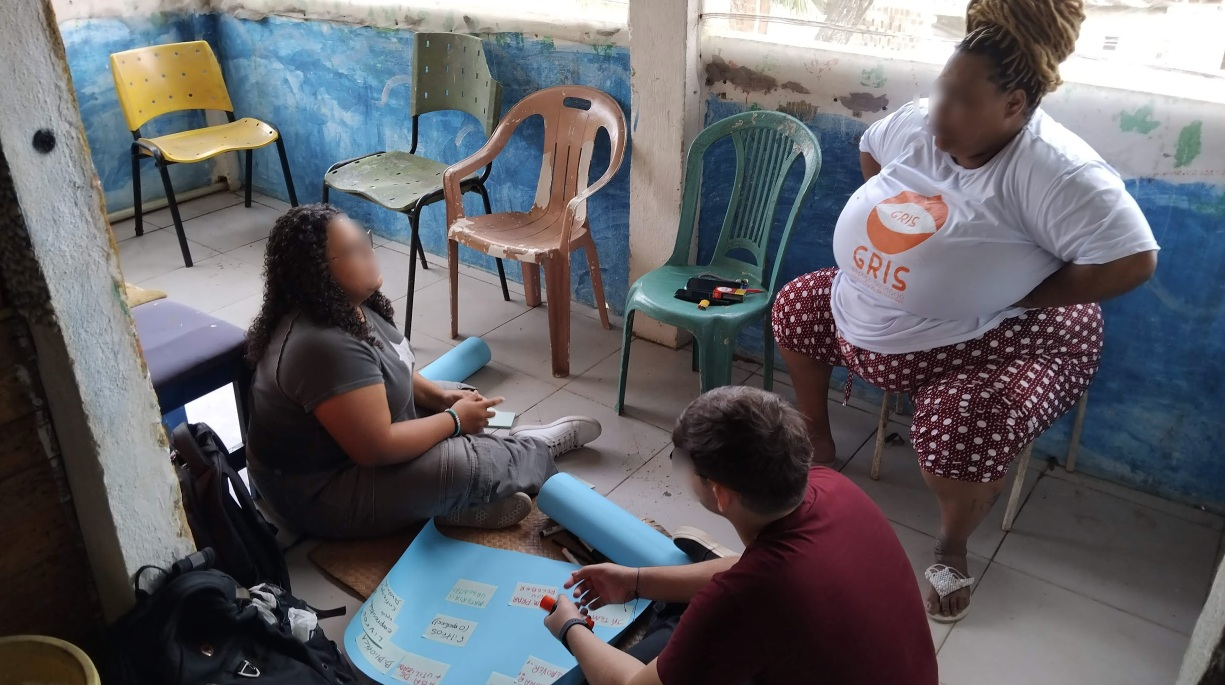
\includegraphics[width=0.6\linewidth]{images/metodologia/ong001.jpeg}
    \label{fig:ong001}
    \vspace{0.2cm}

{\centering Fonte: O autor (2025). \par}
\end{figure}

\begin{figure}[H]
    \caption{Estudantes realizando prototipação via \textit{Wireframe}}
    \centering
    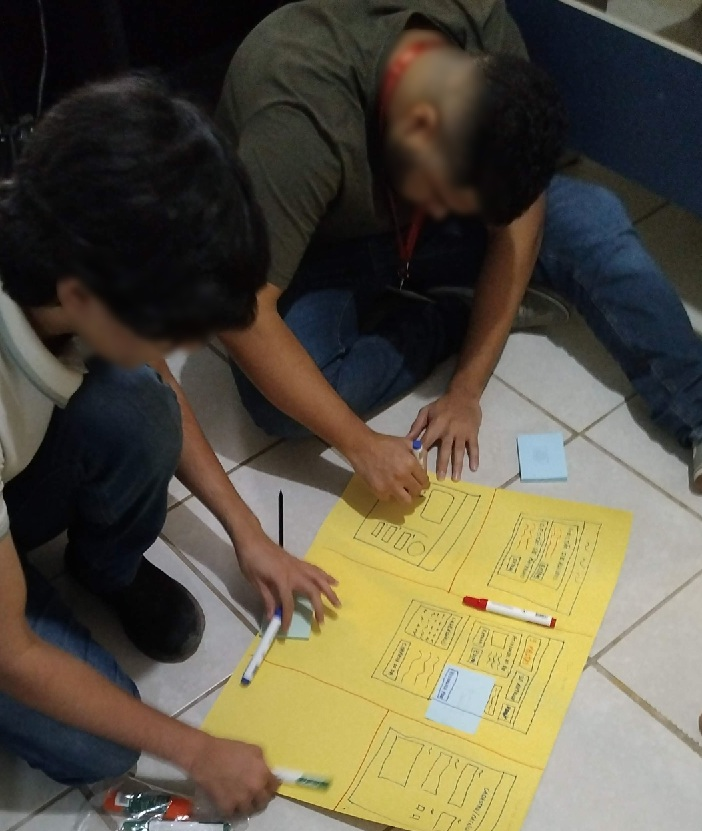
\includegraphics[width=0.6\linewidth]{images/metodologia/ong002.jpeg}
    \label{fig:ong002}
    \vspace{0.2cm}

{\centering Fonte: O autor (2025). \par}
\end{figure}


O cronograma do projeto foi o seguinte, dentro dos quatro ciclos do Speedplay:
\par\vspace{1\baselineskip}

\textbf{Ciclo 1 (Experimentação inicial)}
    \begin{itemize}
        \item Dia 17/08 –\textit{ Prompt-base}
        \item Dia 18 à 20/08 – \textit{Sprint} 1 - Início do \gls{MVP}
        \item Dia 21/08 – \textit{Sprint Review}  - Analisar primeira versão do \gls{MVP} e ajuste do \textit{backlog};
    \end{itemize}
\par\vspace{1\baselineskip}

\textbf{Ciclo 2 (Aprimoramento)}
    \begin{itemize}
        \item Dia 22/08 à 24/08 - \textit{Sprint} 2  - Refinar \gls{MVP} e aplicar as melhorias apontadas na última \textit{Sprint Review}
        \item Dia 25/08 - \textit{Sprint Review} - Verificar a aplicação das melhorias realizadas
        \item Dia 26/08 à 28/08 - \textit{Sprint} 3 - Refinamento do \gls{MVP} e adição de funcionalidades
        \item Dia 29/08 - \textit{Status Report} 1 - Verificação de atendimento de requisitos com \gls{ONG}
    \end{itemize}
\par\vspace{1\baselineskip}

\textbf{Ciclo 3 (Validação e Iteração)}
    \begin{itemize}
        \item Dia 30/08 à 01/09 - \textit{Sprint} 4 - Refinamento do \gls{MVP} e adição de funcionalidades
        \item Dia 02/09 - \textit{Sprint Review} - \textit{Feedback} acerca do \gls{MVP}
        \item Dia 03/09 à 05/09 - \textit{Sprint} 5 - Ajustes e incrementos finais
        \item Dia 06/09 - \textit{Status Report} 2 - Validação do \gls{MVP}
    \end{itemize}
\par\vspace{1\baselineskip}

\textbf{Ciclo 4 (Fechamento e Entrega)}
    \begin{itemize}
        \item Dia 07/09 à 09/09 - \textit{Sprint} 6 - Finalização do \gls{MVP} e preparação para apresentação final
        \item Dia 10/09 - \textit{Sprint Review} - Verificação de últimos ajustes finos e correções na interface
        \item Dia 11/09 à 12/09 - \textit{Sprint} final - Ajustes verificados na última SR
        \item Dia 13/09 - Apresentação final no Espaço \textit{Pitch} - \gls{CIn}/\gls{UFPE}
    \end{itemize}

O projeto contou com a participação direta de seis estudantes do curso de Sistemas de Informação, como equipe responsável pelo desenvolvimento do artefato digital, duas colaboradoras da GRIS Solidário como fonte de informação, participantes da co-criação e validação, o professor orientador auxiliando no processo metodológico e dois pesquisadores na coordenação, coordenando o processo extensionista, e realizando mentoria com os estudantes e alinhamentos necessários com a \gls{ONG}.

Apesar das datas programadas, algumas vezes, a \gls{ONG} teve uma dificuldade em manter as datas agendadas, por conta de adversidades, um quantitativo reduzido de voluntários, onde a própria coordenadora da \gls{ONG} se desdobrou diversas vezes para executar diversas tarefas diferentes na instituição.